% Figure 1: Morphospace and Fitness Landscape (panels A + B)

\begin{figure*}[!t]
\centering

\begin{minipage}[t]{0.48\textwidth}
\centering
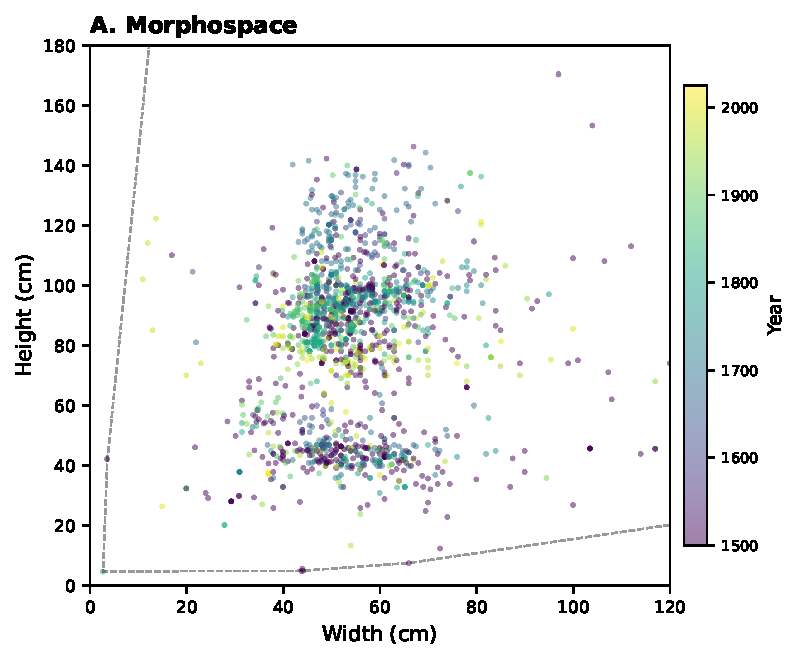
\includegraphics[width=\textwidth]{figures/fig-morphospace-nn.pdf}
\end{minipage}%
\hfill
\begin{minipage}[t]{0.48\textwidth}
\centering
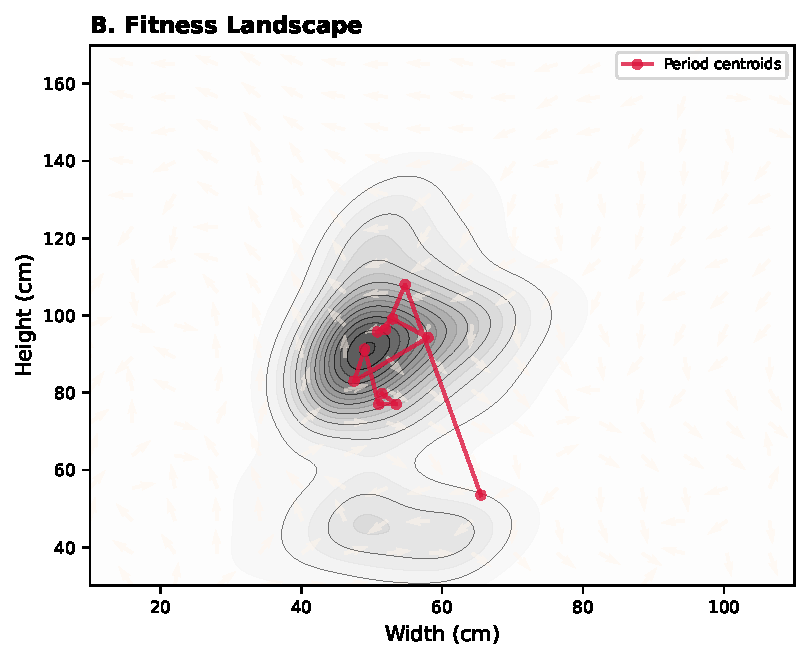
\includegraphics[width=\textwidth]{figures/fig-landscape-nn.pdf}
\end{minipage}

\caption{\textbf{A}: 1\,662 europeiske stolar projiserte i morforommet (breidde $\times$ høgde); farge kodar dato. \textbf{B}: Tilpassingslandskapet som kjernetettleiksestimat med gradientvektorfelt og periodesentriod-trajektorie (raud).}
\label{fig:morphospace}
\end{figure*}
